% from the submitted version (lines 364-406), revised
\subsection{Tracking}
Table~\ref{tab:track} reports ByteTrack on the held-out 15--30\,s with default and tuned parameters. With
default parameters the HOTA difference (\yolo{} minus \rfdetr) is \BtDefGap; \rfdetr{} needs a higher score cut
(\BtMinConfRf{} vs.\ \BtMinConfYolo), after which the difference is \BtTunGap{}---of the order of search
noise. The six-tracker comparison (Fig.~\ref{fig:track}) is more informative: \yolo{} scores higher in
\TcWinsAll{} of \TcPairs{} tracker$\times$GT combinations (\TcWinsOcGt/6 against the OC-SORT-linked GT,
\TcWinsBtGt/6 against the ByteTrack-linked GT), but never by more than \TcMaxGap{} HOTA. Within one detector the
six trackers span at most \TcSpreadBtGt{} (ByteTrack-GT) and \TcSpreadOcGt{} (OC-SORT-GT) HOTA, so the tracker
choice matters little in this scene. The absolute HOTA depends strongly on how the GT was linked (mean
\TcMeanYoloBtGt{} vs.\ \TcMeanYoloOcGt{} for \yolo), so models must only be compared under the same GT.

\begin{table}[t]
\centering
\caption{ByteTrack on the held-out 15--30\,s (pseudo-GT linked by ByteTrack; \BtGtIds{} GT identities). Tuned
parameters were selected on 0--15\,s.}
\label{tab:track}
\footnotesize
\setlength{\tabcolsep}{2.2pt}
\begin{tabular}{llccccccc}
\toprule
Detector & Params & HOTA & MOTA & IDF1 & DetA & AssA & IDSW & IDs \\
\midrule
\multirow{2}{*}{\yolo} & default & \BtHotaYoloDef & \BtMotaYoloDef & \BtIdfYoloDef & \BtDetaYoloDef & \BtAssaYoloDef & \BtIdswYoloDef & \BtIdsYoloDef \\
 & tuned & \BtHotaYoloTun & \BtMotaYoloTun & \BtIdfYoloTun & \BtDetaYoloTun & \BtAssaYoloTun & \BtIdswYoloTun & \BtIdsYoloTun \\
\midrule
\multirow{2}{*}{\rfdetr} & default & \BtHotaRfDef & \BtMotaRfDef & \BtIdfRfDef & \BtDetaRfDef & \BtAssaRfDef & \BtIdswRfDef & \BtIdsRfDef \\
 & tuned & \BtHotaRfTun & \BtMotaRfTun & \BtIdfRfTun & \BtDetaRfTun & \BtAssaRfTun & \BtIdswRfTun & \BtIdsRfTun \\
\bottomrule
\end{tabular}
\end{table}

\begin{figure}[t]
\centering
\figif{fig_tracking.pdf}{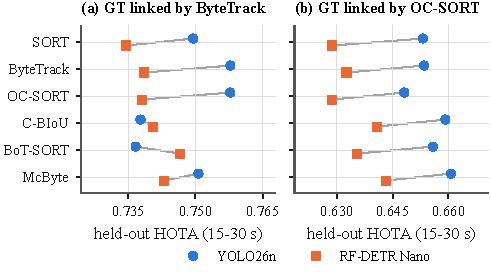
\includegraphics[width=\columnwidth]{figures/fig_tracking.pdf}}
\caption{Held-out HOTA of six trackers per detector, against pseudo-GTs linked by (a) ByteTrack and (b) OC-SORT.
Note the different x-ranges: GT linking shifts all scores.}
\label{fig:track}
\end{figure}

\textbf{Caveats.} The aa1 evaluation window is only 15\,s, and \GridSize{} configurations were searched on the
15\,s before it, so the tuned parameters may fit that window. Both concerns are tested below on longer, unseen
videos with every parameter frozen: the 298\,s held-out video (Sec.~\ref{sec:heldout}) and the two 200\,s campus
scenes (Sec.~\ref{sec:adapt}), where the tuned parameters are also compared with ByteTrack's defaults.

\textbf{Crowd analytics.} Over the first 30\,s, tracks of at least 0.25\,s give \AnUniqueYolo{} unique IDs
for \yolo{} (\AnOverYolo{} vs.\ \AnGtUnique{} in the pseudo-GT) and \AnUniqueRf{} for \rfdetr{}
(\AnOverRf); without the length filter \yolo{} produces \AnRawYolo{} raw IDs. Mean / max occupancy is
\AnMeanYolo{} / \AnMaxYolo{} and the median dwell \AnDwellMedYolo\,s. Unique IDs are an upper bound on people.
